\documentclass[matan]{subfiles}

\begin{document}
  \newpage
  \section{Формула Ньютона-Лейбница. Теорема об интеграле с переменным верхним пределом.}

  \begin{Definition}
  	\[E \subset \R, \q F : E \to \R \q f : E \to \R\]
  	\[\text{Тогда } F \text{ называется первообразной f, если } F'(x) = f(x) \q \forall  x \in  E\]
  \end{Definition}

  \begin{utv}
      $F_1, F_2$ - первообразные $f$ на $E$, тогда:
      $$F(x_1)-F(x_2)=\const \text{ (т. Лагранжа)}$$
  \end{utv}

  \begin{Theorem} [формула Ньютона-Лейбница]
      \[f \in R[a,b],\text{ F -первообразная f, тогда:}\]
      $$\int\limits_a^b f = F(b) - F(a) = F |_a^b$$
  \end{Theorem}

  \begin{proof}
      $\forall \uptau$ на $[a,b]$ по теореме Лагранжа:
      $$\e \xi_k \in [x_k, x_{x+1}]:\ F(x_{k+1})-F(x_k) = F'(\xi_k)(x_{k+1}-x_k) = f(\xi_k) \Delta_k$$
      \\
      Так как $f \in R[a,b] \Rightarrow \forall \E > 0\ \e \updelta > 0: \forall \uptau: \ \uplambda(\uptau) < \updelta,\ \forall \xi \ |S(f, \uptau, \xi) - I| < \E$
      \\
      Возьмём оснащение $\xi$ из теоремы Лагранжа:
      $$S(f, \uptau, \xi) = \sum\limits_{k=0}^{n-1} f(\xi_k) \Delta_k = \sum\limits_{k=0}^{n-1} (F(x_{k+1})-F(x_k)) = F(b) - F(a)$$
  \end{proof}

  \begin{definition}
      $E \subset \R$, \q E - невырожденный промежуток,
  	\[f : E \to  \R \q \forall \alpha, \beta \in E : \q \alpha < \beta \q f \in R[\alpha, \beta] \q \text{ для }a \in E
  	\text{ (фиксированного)}\]
  	\[F(x):=\int\limits_a^x f(t) dt \text{ - интеграл с переменным верхним пределом}\]
  	\[F : E \to \R\]
  \end{definition}

  \begin{theorem}
      $f \in R[a,b],\ F(x) = \int\limits_a^x f(t) dt$, тогда:
      \begin{enumerate}
          \item $F \in C[a,b]$
          \item (теорема Барроу) Если $f$ - непр. в т. $x_0 \in [a,b]$, то $F'(x_0)=f(x_0)$
      \end{enumerate}
  \end{theorem}

  \begin{proof}
      $x \in [a,b],\ h:x+h \in [a,b]$
      \\
      1) $F(x+h)-F(x)= \int\limits_a^{x+h} f - \int\limits_a^x f = \int\limits_a^{x+h} f + \int\limits_x^a f = \int\limits_x^{x+h} f$

      Так как $f \in R[a,b] \Rightarrow \e M \in \R: |f|< M$, значит:
      \[\abs{F(x + h) - F(x)} \leq \abs{\int_x^{x + h} f } \leq \int_x^{x + h}\abs{f} \leq M \abs{h} \]
      Кроме того, $\forall \E > 0,\ \updelta = \frac{\E}{M}$ если $|h| < \updelta \Rightarrow |F(x+h)-F(x)|  < \E$
      \\
  2) Рассмотрим $\abs{\frac{F(x_0+h)-F(x_0)}{h}-f(x_0)} =|\frac{1}{h} \int\limits_{x_0}^{x_0+h} f(t) dt - f(x_0) \frac{1}{h} \int\limits_{x_0}^{x_0+h} dt| =$

      $=\frac{1}{|h|} |\int\limits_{x_0}^{x_0+h} (f(t)-f(x_0)) dt| \leqslant \frac{1}{|h|}|\int\limits_{x_0}^{x_0+h} \E dt| = \E$

      (при $|h| < \updelta\ \forall \E > 0\ \e \updelta > 0: |t-x_0|<\updelta \Rightarrow |f(t)-f(x_0)|< \E$)
  \end{proof}

  \begin{Consequence}
      \[f \in C[a,b] \Rightarrow \e F: F'(x)=f(x)\ \forall x \in [a,b]\]
  \end{Consequence}

  \begin{example}
      $f(x) = |x|,\ F(x) = \int\limits_0^x |t| dt =
       \begin{cases}
         \dfrac{t^2}{2} \Big|_0^x,& x \geqslant 0\\
         \\
         -\dfrac{t^2}{2} \Big|_0^x,& x < 0
       \end{cases}$
  \end{example}

  \begin{example}
      $f(x) =
       \begin{cases}
         1,& x \geqslant 0
         \\
         -1,& x < 0
       \end{cases}$

      $F(x) = |x| \ \forall x \neq 0$, видно что неверно для первообразной, но:
      \begin{definition}
          F - "почти первообразная"$,$ если:
          \begin{enumerate}
              \item $F'(x) = f(x)\ \forall x \in [a,b] \setminus \{t_1, ... t_n\}$
              \item $F \in C[a,b]$
          \end{enumerate}
      \end{definition}

      \begin{example}
          Пример для "почти первообразной". Найти $\int\limits_0^2 f(x)$, для $f(x) = \max(1,x)$

          $F(t) \os{?}{=}
           \begin{cases}
             t,& t \in [0,1]
             \\
             \frac{t^2}{2},& t \in [1,2]
           \end{cases}$

          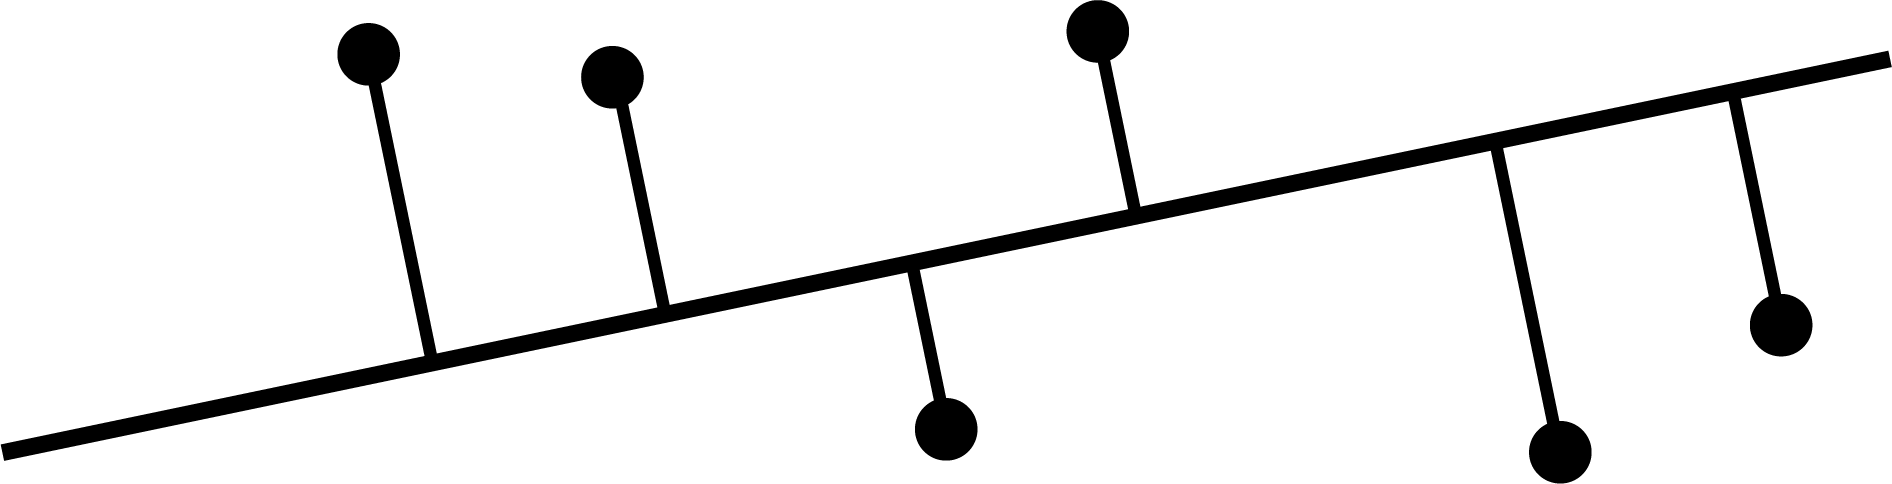
\includegraphics[scale=0.5]{11_1}

          Попробуем использовать Н-Л: $F(t) \big|_0^2 = F(2) - F(0) = 2$ \\Неверно, потому что это не первообразная и даже не "почти первообразная". Поправим F(x):

          $F(t) =
           \begin{cases}
             t,& t \in [0,1]
             \\
             \frac{t^2}{2} + \frac{1}{2},& t \in [1,2]
           \end{cases}$

          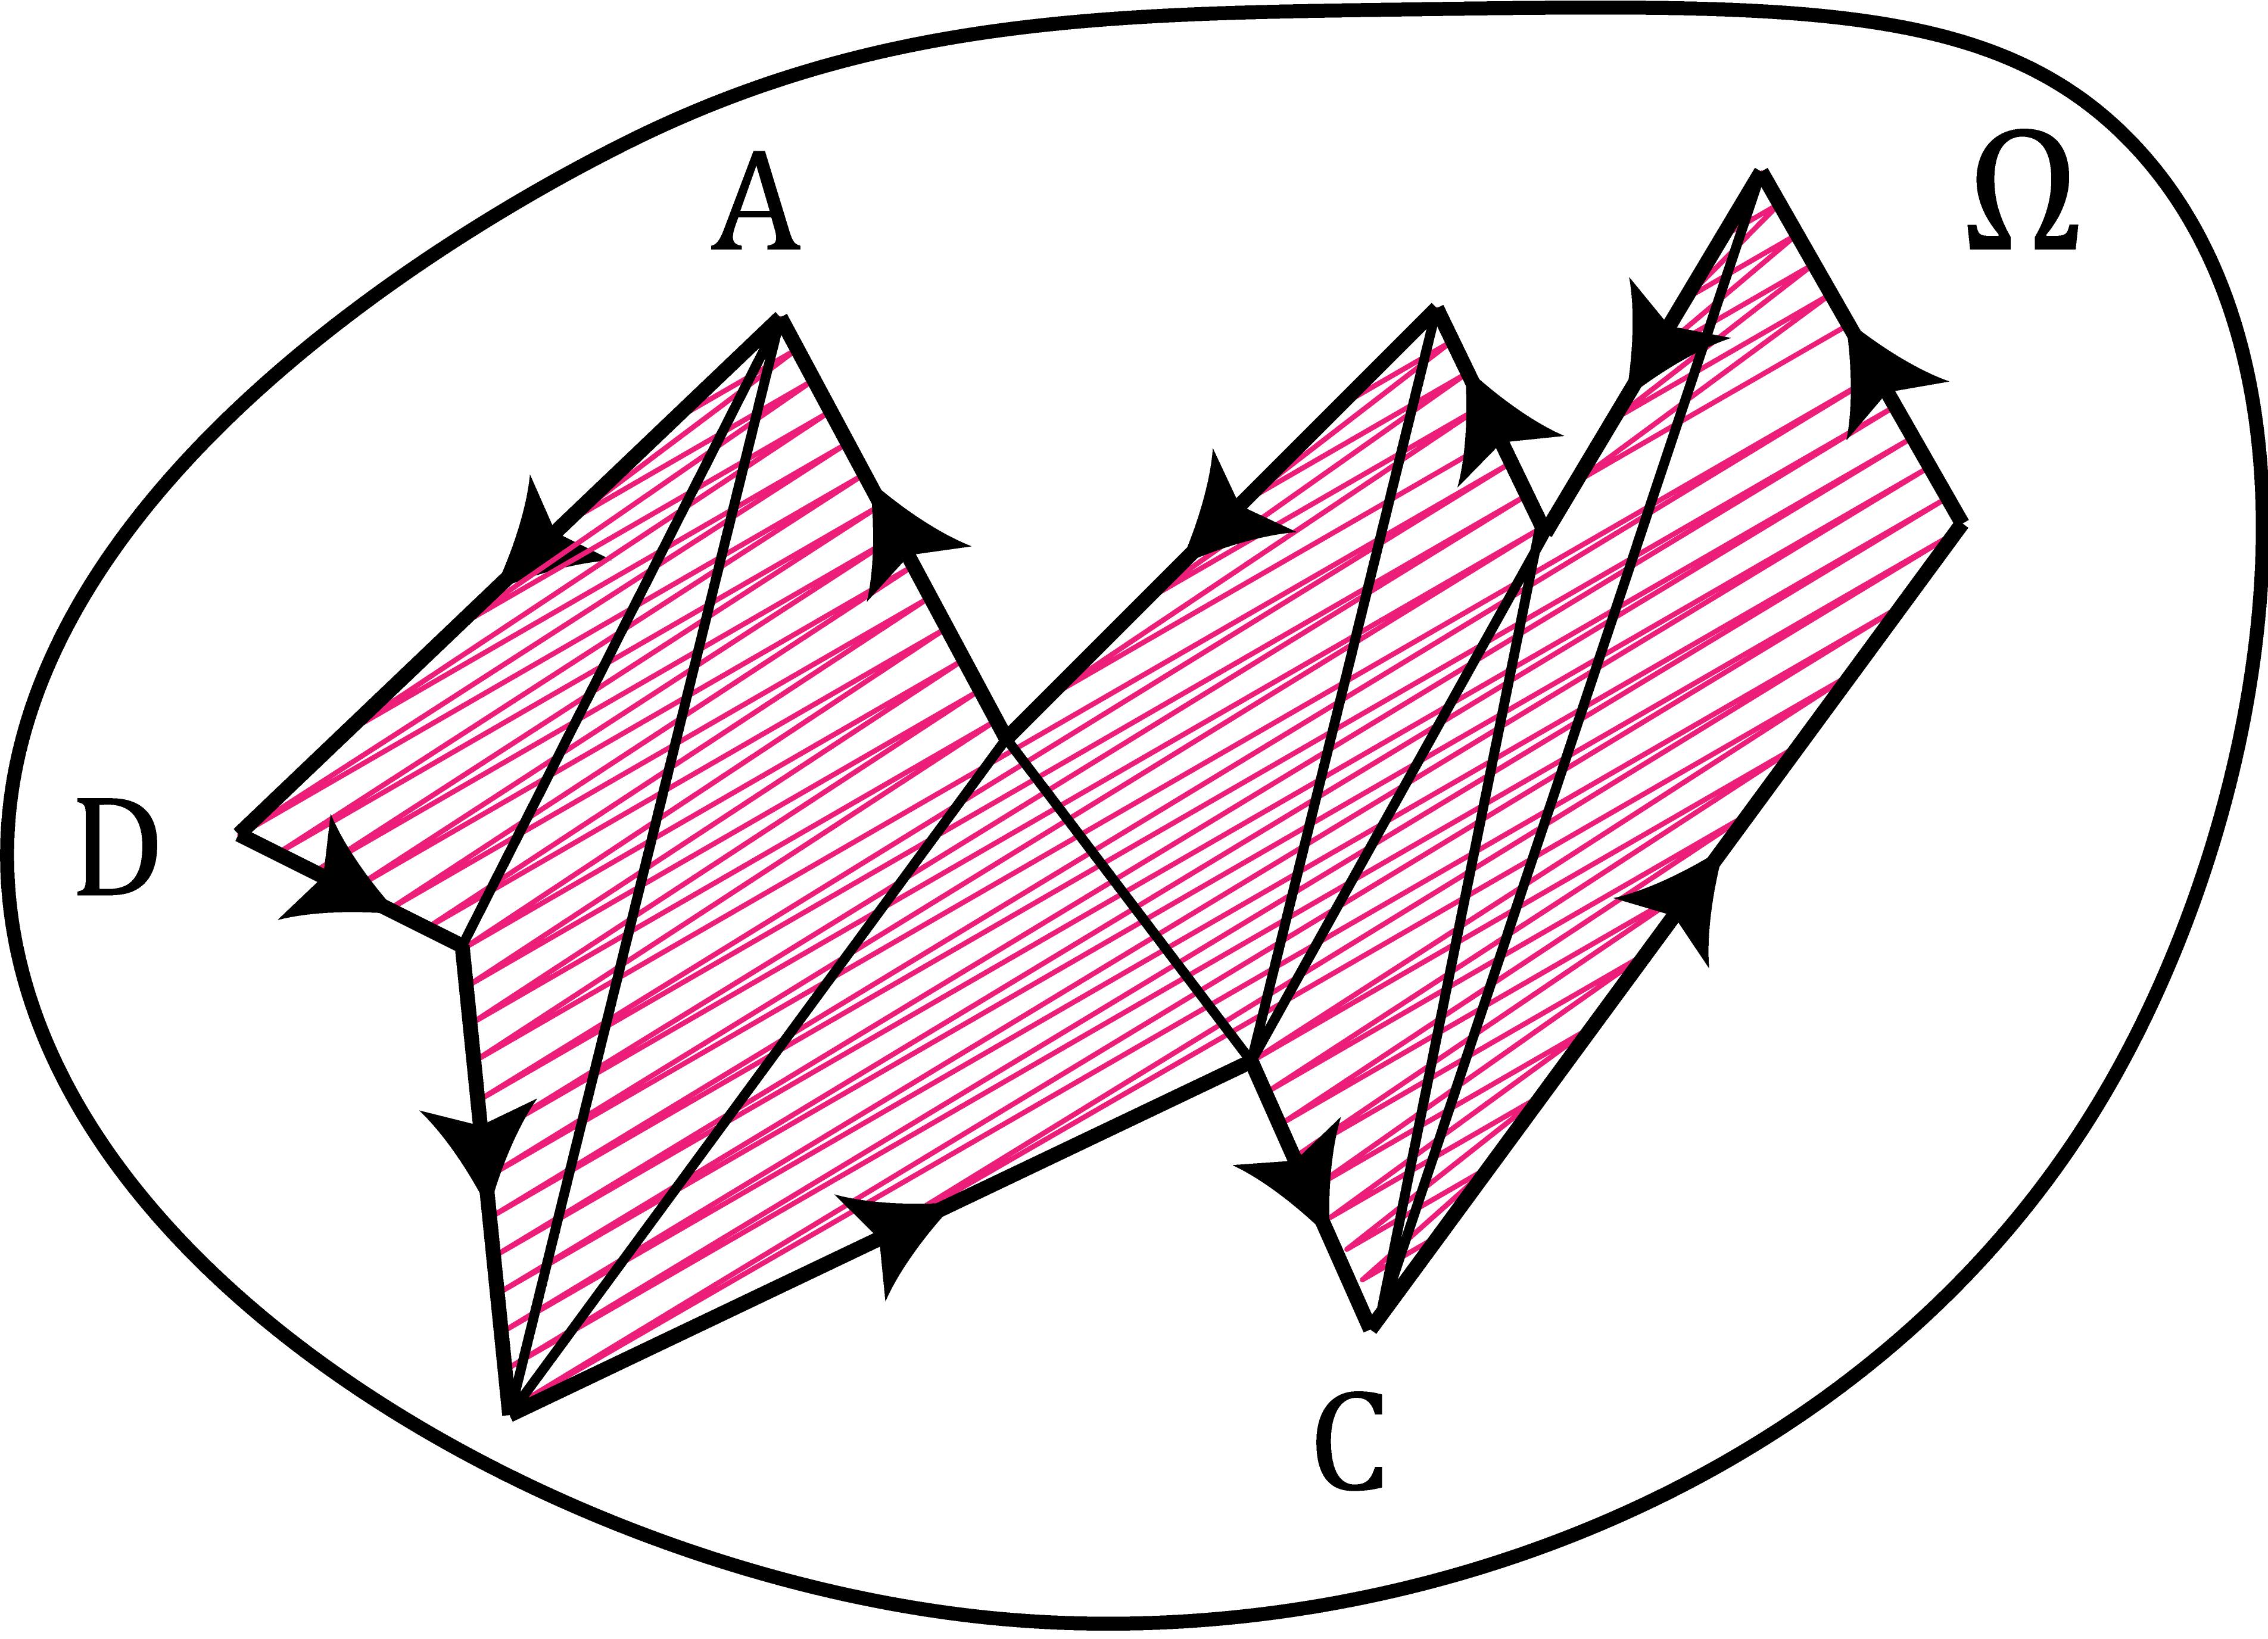
\includegraphics[scale=0.5]{11_2}

          Это уже "почти первообразная"\ можно применять Н-Л.
      \end{example}
  \end{example}

  \newpage
  \section{Формула интегрирования по частям в интеграле Римана. Применение: формула Валлиса.}
  \hypertarget{12q}{}
  \begin{Theorem}
      \[\text{$F,G$ - первообразные $f,g \in R[a,b]$ на $[a,b]$, тогда } \int\limits_a^b F g = F G |_a^b-\int\limits_a^b f G\]
      $$(\int\limits_a^b u v' = u v |_a^b - \int\limits_a^b u' v)$$
  \end{Theorem}

  \begin{Proof}
      \[(F G)' = f G + F g, \text{ по ф-ле Н-Л: }\int\limits_a^b (F G)' =
      F G |_a^b = \int\limits_a^b f G + \int\limits_a^b F g\]
  \end{Proof}

  \begin{example}
      Если $I_m := \int\limits_0^{\frac{\pi}{2}} \sin^m x dx = \int\limits_0^{\frac{\pi}{2}} \cos^m x dx$, то:

      \[
      I_m =
       \begin{cases}
         \dfrac{\pi}{2} \dfrac{(m-1)!!}{m!!}, &\text{$m$ - четное}\\ \\
         \dfrac{(m-1)!!}{m!!}, &\text{$m$ - нечетное}
       \end{cases}
      \]
  \end{example}

  \begin{Proof}
      \begin{multline*}
          $$I_m = \int\limits_0^{\frac{\pi}{2}} \sin^m x dx = \int\limits_0^{\frac{\pi}{2}} (-\cos x)' \sin^{m-1} x dx =\\= - \cos x \sin^{m-1} x |_0^{\frac{\pi}{2}} - \int\limits_0^{\frac{\pi}{2}} \cos^2 x (m-1) \sin^{m-2} x dx =\\= (m-1) \int\limits_0^{\frac{\pi}{2}} (\sin^{m-2} x - \sin^m x) dx = (m-1)(I_{m-2}-I_m)$$
      \end{multline*}

      \[I_m=\frac{m-1}{m} I_{m-2},\ I_0=\frac{\pi}{2},\ I_1= 1,\ I_2=\frac{\pi}{2} \frac{1}{2},\ I_{2k}=\frac{\pi}{2} \frac{1}{2} \frac{3}{4} ... \frac{2k-1}{2k} = \frac{\pi}{2} \frac{(2k-1)!!}{(2k)!!}\]
  \end{Proof}

  \begin{Theorem}[Формула Валлиса]
      \[\lim\limits_{n \rightarrow \infty} \frac{2*2*4*4*...*(2n)(2n)}{1*3*3*5*5...(2n-1)(2n+1)} = \dfrac{\pi}{2}$ (или $\lim\limits_{n \rightarrow \infty} \frac{1}{n} (\frac{(2n)!!}{(2n-1)!!})^2 = \pi)\]
  \end{Theorem}

  \begin{proof}
      $\forall x \in [0, \frac{\pi}{2}]$ верно $\int\limits_0^{\frac{\pi}{2}} \sin^{2n+1} x \leqslant \int\limits_0^{\frac{\pi}{2}} \sin^{2n} x \leqslant \int\limits_0^{\frac{\pi}{2}} \sin^{2n-1} x$
      $$\frac{(2n)!!}{(2n+1)!!} \leqslant \frac{\pi}{2} \frac{(2n-1)!!}{(2n)!!} \leqslant \frac{(2n-2)!!}{(2n-1)!!}$$
      $$A_n=\frac{((2n)!!)^2}{(2n-1)!!(2n+1)!!} \leqslant \frac{\pi}{2} \leqslant \frac{(2n)!! (2n-2)!!}{((2n-1)!!)^2}=B_n$$
      \begin{multline*}
          $$B_n - A_n = \frac{(2n)!! (2n-2)!!}{((2n-1)!!)^2} - \frac{((2n)!!)^2}{(2n-1)!!(2n+1)!!} =\\= (\frac{(2n)!!}{(2n-1)!!})^2 (\frac{1}{2n} - \frac{1}{2n+1})=(\frac{((2n)!!)^2}{(2n-1)!!(2n-1)!!})\frac{1}{(2n+1)(2n)}=\\
          =A_n \frac{1}{2n} \leqslant \frac{\pi}{2} \frac{1}{2n} \rightarrow\limits_{n \rightarrow \infty} 0 \Rightarrow \lim\limits_{n \rightarrow \infty} A_n = \lim\limits_{n \rightarrow \infty} B_n=\frac{\pi}{2}$$
      \end{multline*}
  \end{proof}

  \newpage
  \section{Формула Тейлора с остаточным членом в интегральной форме.}

  \begin{Theorem}
      \begin{multline*}
          $$f \in C^{n+1} ([a,b]) \Rightarrow f(b)=\sum\limits_{k=0}^n \frac{f^{(k)}(a)}{k!} (b-a)^k + R_n (b,a), \\ \text{ где }R_n(b,a)=\frac{1}{n!} \int\limits_a^b f^{(n+1)}(t) (b-t)^n dt$$
      \end{multline*}
  \end{Theorem}

  \begin{Remark}
      \[f \in C^{n+1}([a,b]) \Rightarrow f^{(n+1)} \in C[a,b] \Rightarrow \e \xi \in [a,b]:\]
      \[R_n=\frac{1}{n!} f^{(n+1)} (\xi) \int\limits_a^b(b-t)^n dt = \frac{-f^{(n+1)}(\xi)}{n!} \frac{(b-t)^{n+1}}{n+1} \Big|_a^b = \frac{f^{(n+1)}(\xi)}{(n+1)!} (b-a)^{n+1}\]
  \end{Remark}

  \begin{proof}[по индукции]
      1) $n=0$

      $f(b)=f(a)+\int\limits_a^b f'(t) dt$ - формула Н-Л
      \\
      2) Инд. переход. Пусть для $n-1$ - доказано, $f \in C^{n-1}[a,b] \subset C^n [a,b]$, по инд. предположению:
      $$f(b)=\sum\limits_{k=0}^{n-1} \frac{f^{(k)}(a)}{k!} (b-a)^k + R_{n-1} (*)$$
      $$R_{n-1} = \frac{1}{(n-1)!} \int\limits_a^b f^{(n)}(t) (b-t)^{n-1} dt =
      \begin{bmatrix}
      u=f^{(n)}(t)\\
      v'=(b-t)^{n-1}
      \end{bmatrix} = $$
      $$= \frac{1}{(n-1)!} (-f^{(n)}(t)\frac{(b-t)^n}{n}\bigg|_a^b + \int\limits_a^b f^{(n+1)}(t)\frac{(b-t)^n}{n} dt) = $$
      $$=\frac{1}{(n)!} (f^{(n)}(a)(b-a)^n+ \int\limits_a^b f^{(n+1)}(t)(b-t)^n dt)\text{ - подставить в $(*)$}$$
  \end{proof}

  \newpage
  \section{Формула интегрирования по частям в интеграле Римана. Вторая теорема о среднем.}

  Формулу интегрирования по частям см. в  \hyperlink{12q}{12 билете.}
  \begin{Theorem}[Бонне или вторая теорема о среднем]
      \begin{multline*}
          $$f \in C[a,b],\ g\in C^1[a,b], g - \text{монотонна} \\
          \Rightarrow \e \xi \in [a,b]: \int\limits_a^b f g = g(a) \int\limits_a^\xi f  + g(b) \int\limits_\xi^b f$$
      \end{multline*}
  \end{Theorem}

  \begin{proof}
      (для $g\nearrow$) $F(x):=\int\limits_a^x f \Rightarrow F'=f$
      $$\int\limits_a^b f g = \int\limits_a^b F' g = F g |_a^b - \int\limits_a^b F g' = F(b)g(b) - F(a)g(a) - \int\limits_a^b F g' = $$
      $$\text{(т.к. $g\nearrow$ $g' \geqslant 0 \Rightarrow$ по т. о среднем $\e \xi \in [a,b]:)$}$$
      $$= F(b) g(b) -  g(a) F(a) - F(\xi)\int\limits_a^b g' = g(b)(F(b)-F(\xi))+g(a)(F(\xi)-F(a))$$
  \end{proof}

  \newpage
  \section{Замена переменной в определенном интеграле (две формулировки, доказательство одной).}


  \begin{Theorem}
      \[\upvarphi \subset C^1 [\upalpha,\upbeta],\ f \in C(\upvarphi([\upalpha,\upbeta])),\text{ тогда } \int\limits_{\upvarphi(\upalpha)}^{\upvarphi(\upbeta)} f = \int\limits_{\upalpha}^{\upbeta} (f \circ \upvarphi) \upvarphi'\]
  \end{Theorem}

  \begin{proof}
      $f \in C(\upvarphi([\upalpha,\upbeta])) \Rightarrow \e F: F'=f$
      $$(F \circ \upvarphi)' = (F' \circ \upvarphi) \upvarphi' = (f \circ \upvarphi) \upvarphi' \Rightarrow \int\limits_\upalpha^\upbeta (f \circ \upvarphi) \upvarphi' =( F \circ \upvarphi) (\upbeta) - (F \circ \upvarphi) (\upalpha)$$
      $$ \int\limits_{\upvarphi(\upalpha)}^{\upvarphi(\upbeta)} f = F(\upvarphi(\upbeta)) - F(\upvarphi(\upalpha)) = \int\limits_\upalpha^\upbeta (f \circ \upvarphi) \upvarphi'$$
  \end{proof}

  \begin{Theorem}
      \begin{multline*}
          $$f \in R[a,b],\ \upvarphi \in C^1 [\upalpha, \upbeta],\ \upvarphi \text{ - строго возрастает}, \\
          \upvarphi(\upalpha) = a,\q \upvarphi(\upbeta) = b,
          \text{ тогда } \int\limits_a^b f = \int\limits_\upalpha^\upbeta (f \circ \upvarphi) \upvarphi'$$
      \end{multline*}
  \end{Theorem}

  \begin{Example}
      \[\int\limits_0^1 \sqrt{1-x^2} dx,\q \upvarphi(t) = \cos t,\q \upvarphi(\upalpha)=0$, $\upvarphi(\upbeta)=1\]

      \[\int\limits_0^1 \sqrt{1-x^2} dx = - \int\limits_{\frac{\pi}{2}}^0 \sqrt{1-\cos^2 t} \sin t dt = - \int\limits_{\frac{\pi}{2}}^0 \frac{1 - \cos 2t}{2} dt = (-\frac{t}{2} + \frac{\sin 2t}{4}) \Big|_{\frac{\pi}{2}}^0 = \frac{\pi}{4}\]
  \end{Example}

  \newpage
  \begin{Reminder} [про ряды]\
  \begin{definition}
      Числовой ряд из элементов $\{a_j\}_{j \in \N}$ - это $\sum\limits_{j=1}^\infty a_j$
  \end{definition}

  \begin{definition}
      Частичная сумма ряда $S_n = \sum\limits_{j=1}^n a_j$
  \end{definition}

  \begin{definition}
      Говорят, что сумма ряда $S=\sum\limits_{j=1}^\infty a_j=\lim\limits_{n \rightarrow \infty} S_n$
  \end{definition}

  \begin{Remark}
      \[\text{Ряд $\sum\limits_{j=1}^\infty a_j$ сходится или расходится одновременно с рядом $\sum\limits_{j=N}^\infty a_j$}\]
  \end{Remark}

  \begin{Theorem} [необходимое условие сходимости]
      \[\text{Если $\sum\limits_{j=1}^\infty a_j$ - cходится, то $\lim\limits_{j \rightarrow \infty} a_j = 0$}\]
  \end{Theorem}

  \begin{definition}
      Ряд Лейбница $\sum\limits_{j=0}^\infty (-1)^j a_j$, $a_j>0$, где $\lim\limits_{j \rightarrow \infty} a_j =0$, $a_j \searrow$
  \end{definition}

  \begin{theorem}\ \\
      Пусть $\sum\limits_{j=0}^\infty (-1)^j a_j$ - ряд Лейбница, тогда:
      \begin{enumerate}
          \item Ряд Лейбница сходится
          \item $S_{2n} \searrow$, $S_{2n-1} \nearrow$
          \item $|S-S_n|<a_{n+1}$
      \end{enumerate}
  \end{theorem}

  \begin{theorem}\ \\
      Критерий Коши для числовых последовательностей.

      $\sum\limits_{j=1}^\infty a_j$ - сх $\lra \forall \E > 0\ \e N: \forall m>n>N\ |S_m-S_n|<\E$
  \end{theorem}
  \end{Reminder}

  \newpage
  \section{Признаки сравнения для положительных рядов.}

  \begin{definition}
      Если $a_j \geqslant 0$, то $\sum\limits_{j=1}^\infty a_j$ - положительный ряд
  \end{definition}

  \begin{theorem}\ \\
      Положительный ряд сходится $\lra S_n$ - ограничены
  \end{theorem}

  \begin{consequence} \ \\
      Пусть $0 \leqslant a_j \leqslant b_j$, тогда:
      \begin{enumerate}
          \item $\sum b_j$ - сх $\Rightarrow$ $\sum a_j$ - сх (первый признак сходимости)
          \item $\sum a_j$ - расх $\Rightarrow$ $\sum b_j$ - расх (первый признак сравнения)
      \end{enumerate}
  \end{consequence}

  \begin{Consequence}
      \[a_k \geqslant 0,\ b_k \geqslant 0,\ \e c,d > 0\ \e N: \forall n > N\ 0 < c \leqslant \frac{a_n}{b_n} \leqslant d \leqslant \infty\]
      Тогда $\sum a_k$ и $\sum b_k$ сх. или расх. одновременно
  \end{Consequence}

  \begin{proof}
      (т.е. $\sum a_k$ - сх $\lra$ $\sum b_k$ - сх)

      ($\Leftarrow$) $0 \leqslant a_n \leqslant d b_n$ т.к. $d b_n$ - сх $\Rightarrow$ $a_n$ - сх

      ($\Rightarrow$) $0 \leqslant c b_n \leqslant a_n$ т.к. $a_n$ - сх $\Rightarrow$ $c b_n$ - сх $\Rightarrow$ $b_n$ - сх
  \end{proof}

  \begin{consequence} [второй признак сравнения]
      Пусть $a_n, b_n \geqslant 0$, тогда если

      $\e \lim\limits_{n \rightarrow \infty} \dfrac{a_n}{b_n} = L \in (0, + \infty)$, то $\sum a_n$ и $\sum b_n$ сх или расх одновременно
  \end{consequence}

  \begin{proof}
      Возьмём $\E:=\dfrac{L}{2} \Rightarrow \e N: \forall n > N$ $\big|\dfrac{a_n}{b_n} - L\big| < \dfrac{L}{2} \Rightarrow$

      $0 < \dfrac{L}{2} < \dfrac{a_n}{b_n} < \dfrac{3L}{2} < +\infty \Rightarrow$ по предыдущему следствию верно
  \end{proof}

  \newpage
  \section{Признаки Даламбера и Коши для положительных рядов.}

  \begin{theorem} [радикальный признак Коши для положительных рядов]
      $a_k \geqslant 0$, $c:=\overline{\lim\limits_{k \rightarrow \infty}} \sqrt[k]{a_k}$

      Если $c < 1$, то $\sum a_k$ - сх

      Если $c > 1$, то $\sum a_k$ - расх
  \end{theorem}

  \begin{proof}

      а) $0 \leqslant c < 1$
      \begin{figure}[H]
          \centering
          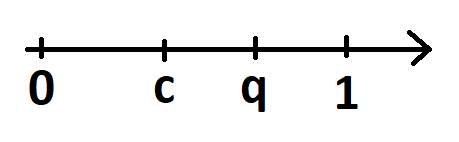
\includegraphics[width=3cm]{pics/17_1}
      \end{figure}
      $q := \frac{c+1}{2}$, $c<q<1$, по характеристике $\overline{\lim}: \e N: \forall n > N\ \sqrt[n]{a_n} < q$

      т.к. $0 \leqslant a_n < q^n$ и $\sum q^n$ - сх $\Rightarrow \sum a_n$ - сх
      \\
      б) $c > 1$
      \begin{figure}[H]
          \centering
          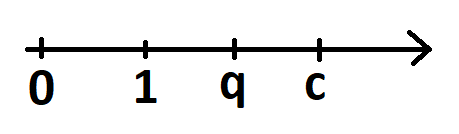
\includegraphics[width=3cm]{pics/17_2}
      \end{figure}
      $q := \frac{c+1}{2}$, $1<q<c$, по характеристике $\overline{\lim}:$ $\forall N: \e n > N$ $\sqrt[n]{a_n} > q$

      т.е. $\e$ бесконечное мн-во $\sqrt[n_k]{a_{n_k}} > q$, $a_{n_k} > q^{n_k} > 1$

      $\Rightarrow \lim a_{n_k} \neq 0 \Rightarrow \sum a_n$ - расх
  \end{proof}

  \begin{theorem} [признак Даламбера сходимости положительных рядов]
      $a_k \geqslant 0$, $\mathcal{D}:=\lim\limits_{k \rightarrow \infty} \frac{a_{k+1}}{a_k}$

      Если $\mathcal{D} < 1$, то $\sum a_k$ - сх

      Если $\mathcal{D} > 1$, то $\sum a_k$ - расх
  \end{theorem}

  \begin{proof}
      а) $\mathcal{D} < 1$, $q := \frac{\mathcal{D} + 1}{2}$ $\E := \frac{1 - \mathcal{D}}{2}$
      \begin{figure}[H]
          \centering
          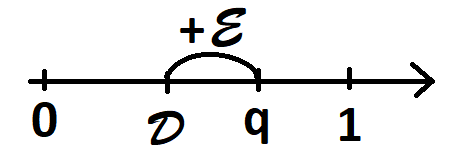
\includegraphics[width=3cm]{pics/17_3}
      \end{figure}
      $\e N: \forall k>N$ $\mathcal{D}-\E < \frac{a_{k+1}}{a_k} < \mathcal{D}+\E = q$ - геом пр. $q < 1$

      $a_{k+1} < q a_k < q^2 a_{k-1} < ... < q^{k-N+1} a_N$, $\sum q^{k-N+1} a_k$ - сх $\Rightarrow \sum a_{k+1}$ - сх по первому пр. сходимости
      \\
      б) $\mathcal{D} < 1$, $q := \frac{\mathcal{D} + 1}{2}$ $\E := \frac{\mathcal{D} - 1}{2}$
      \begin{figure}[H]
          \centering
          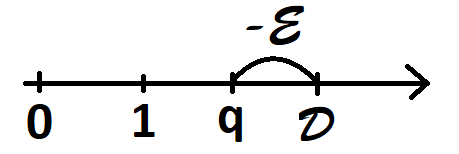
\includegraphics[width=3cm]{pics/17_4}
      \end{figure}
      $\e N: \forall k>N$ $q = \mathcal{D}-\E < \frac{a_{k+1}}{a_k} < \mathcal{D}+\E$, $q > 1$

      $a_{k+1}> q a_k > q^2 a_{k-1} > ... >q^{k-N+1} a_N$, $\sum q^{k-N+1} a_N$ - расх $\Rightarrow \sum a_{k+1}$ - расх по первому пр. сравнения
  \end{proof}

  \newpage
  \section{Абсолютная и условная сходимость рядов. Сходимость следует из абсолютной сходимости.}
  \hypertarget{q18}{}

  \begin{definition}
      $\sum\limits_{j=1}^\infty a_j$ - сх абсолютно, если $\sum\limits_{j=1}^\infty |a_j|$ - сх
  \end{definition}

  \begin{definition}
      Ряд сходится условно если сходится, но не абсолютно
  \end{definition}

  \begin{theorem}
      Если ряд сходится абсолютно, то он сходится
  \end{theorem}

  \begin{proof} \ \\
      $\sum\limits_{j=1}^\infty |a_j|$ - сх, по критерию Коши $\forall \E > 0\ \e N: \forall m>n>N:$

      $$||a_{n+1}|+...+|a_m||<\E \text{, по неравенству треугольника:}$$
      $$|a_{n+1}+...+a_m|<\E \Rightarrow \sum\limits_{j=1}^\infty a_j \text{ - сх.}$$
  \end{proof}

  \newpage
  \section{Абсолютная и условная сходимость. Пример: $\sum\limits_{n=1}^\infty \frac{(-1)^{n-1}}{n}$}

  Определения см. в \hyperlink{q18}{предыдущем} билете. \\
  Ряд не сходится абсолютно, т.к. $\sum\limits_{n=1}^\infty \big|\frac{(-1)^{n-1}}{n}\big|=\sum\limits_{n=1}^\infty \frac{1}{n}$ - расх. ряд, т.к.:

  \begin{theorem} [критерий Коши сходимости последовательности]
      $x_n$ - сх $\lra x_n$ - сх в себе.
  \end{theorem}
  Покажем, что для $S_n=1+\frac{1}{2}+...+\frac{1}{n}$ $\e \E > 0: \forall N\ \e m,n \geqslant N: |x_m-x_n|>\E$:
  $$\text{Возьмём }\E = \frac{1}{4}\text{ n }=N,\ m=2N:$$
  $$|S_{2N} - S_N| = \Big|\frac{1}{N+1}+...+\frac{1}{2N}\Big| > N \frac{1}{2N} = \frac{1}{2} > \E$$ \\
  Но ряд сходится (значит условно сходится) по признаку Лейбница (или это можно показать прямо, доказав что $S_{2n} \nearrow$ и ограничена сверху единицей, а $S_{2n+1}=S_{2n}$ в пределе)

  \newpage
  \section{Перестановка абсолютно сходящегося ряда. Теорема Римана (б/д).}

  \begin{definition}
      Пусть есть ряд $\sum\limits_{k=1}^\infty a_k$ и биективная функция $\upvarphi: \N \rightarrow \N$, тогда ряд $\sum\limits_{k=1}^\infty a_{\upvarphi(k)}$ называется перестановкой ряда $\sum\limits_{k=1}^\infty a_k$
  \end{definition}

  \begin{theorem} [Римана v1] \ \\
      Пусть ряд $\sum a_n$ - условно сходится, тогда:
      \[\forall S \in \overline{\R}\ \e \upvarphi: \N \rightarrow \N: \sum a_{\upvarphi(k)} = S\]
  \end{theorem}

  \begin{definition}
      $a_k^+ = \max\{a_k, 0\}$, $a_k^- = \max\{-a_k, 0\}$
  \end{definition}

  \begin{theorem} [Дирихле, о перестановке абсолютно сходящегося ряда] \ \\
      Если $\sum\limits_{n=1}^\infty a_n= S$ сх абсолютно, то

      $\forall \upvarphi: \N \rightarrow \N$, где $\upvarphi$ - биекция $\Rightarrow \sum\limits_{n=1}^\infty a_{\upvarphi(n)} = S$
  \end{theorem}

  \begin{proof}\\
      а) Пусть $a_n \geqslant 0\ \forall n \in \N$

      $S := \sum\limits_{n=1}^\infty a_n$ - сх $\lra$ все частичные суммы ограничены,  $S_n \leqslant S\ \forall n \in \N$

      Частичные суммы $\sum\limits_{k=1}^n a_{\upvarphi(k)}$ обозначим перестановками ряда $T_n := \sum\limits_{k=1}^n a_{\upvarphi(k)}$

      Пусть $m:=\max \{\upvarphi(1), \upvarphi(2), ..., \upvarphi(n) \}$

      $T_n \leqslant S_m := \sum\limits_{n=1}^m a_{\upvarphi(a_n)} \leqslant S \Rightarrow T_n \nearrow$ - огр $\lra$ ряд $T := \sum\limits_{n=1}^\infty a_{\upvarphi(a_n)}$ сходится.

      Предельный переход даёт $T \leqslant S$, но так как $S$ - тоже перестаовка $T$ $\Rightarrow$ $S \leqslant T$

      Значит $S=T$, то есть $\sum\limits_{n=1}^\infty a_n = \sum\limits_{n=1}^\infty a_{\upvarphi(a_n)}$
      \\
      б) Общий случай, $a_k \in \R $

      $a_k = a_k^+ - a_k^-$, $|a_k| = a_k^+ + a_k^- \Rightarrow a_k^+ = \frac{a_k + |a_k|}{2},\ a_k^-=\frac{|a_k|-a_k}{2}$

      т.к. $\sum a_k$ - сх абсолютно $\Rightarrow \sum |a_k|$ - сх

      $\Rightarrow \sum a_k^+,\ \sum a_k^-$ - сх (причем абсолютно)

      $$\sum\limits_{k=0}^\infty a_{\upvarphi(k)} = \sum\limits_{k=0}^\infty (a_{\upvarphi(k)}^+ - a_{\upvarphi(k)}^-) = \sum\limits_{k=0}^\infty a_{\upvarphi(k)}^+ - \sum\limits_{k=0}^\infty a_{\upvarphi(k)}^- =\text{ (п. а) }\sum\limits_{k=0}^\infty (a_k^+ - a_k^-) = \sum\limits_{k=0}^\infty a_k$$
  \end{proof}

  \begin{theorem} [Римана v2]
      Пусть ряд $\sum a_n$ - условно сходится. Тогда $\sum a_n^+ - \sum a_n^- = + \infty$
  \end{theorem}

  \begin{proof}
      Можно доказать одну из теорем
  \end{proof}
\end{document}
